\documentclass[11pt,a4paper]{article}
\usepackage[T1]{fontenc}
\usepackage[utf8]{inputenc}
\usepackage{lmodern}
\usepackage{textcomp}
\usepackage[left=1.8cm,right=1.8cm,top=2.3cm,bottom=2.2cm,headheight=14pt,headsep=8pt]{geometry}
\usepackage{multicol}
\usepackage{xcolor}
\usepackage{fancyhdr}
\usepackage{graphicx}
\usepackage{array}
\usepackage{amsmath,amssymb}
\usepackage{setspace}
\usepackage{longtable}
\graphicspath{{../}}
\definecolor{ygreen}{RGB}{46,139,87}
\renewcommand{\normalsize}{\fontsize{10.9}{13.4}\selectfont}
\renewcommand{\familydefault}{\rmdefault}
\setlength{\parindent}{0pt}
\setlength{\columnsep}{0.8cm}
\setlength{\columnseprule}{0.4pt}
\setlength{\multicolsep}{3pt plus 1pt minus 1pt}
\renewcommand{\textsubscript}[1]{\ensuremath{_{\text{\fontsize{8}{8}\selectfont #1}}}}
\renewcommand{\textsuperscript}[1]{\ensuremath{^{\text{\fontsize{8}{8}\selectfont #1}}}}
\newcommand{\diqqat}[1]{\par\smallskip\noindent\textbf{Diqqat!} #1\par\medskip}
\newcommand{\javob}{\par\smallskip\noindent\textbf{Javob:} \rule[-2pt]{7.5cm}{0.4pt}\par\smallskip\noindent\textbf{Diqqat!} Javobingizni javoblar varaqasiga ko`chirib yozing.\par\medskip}
\pagestyle{fancy}
\fancyhf{}
\renewcommand{\headrulewidth}{0.4pt}
\fancyhead[L]{\textit{Milliy sertifikat 2026. Kimyo}}
\fancyhead[R]{8-variant}
\fancyfoot[L]{\fontsize{8}{9}\selectfont \textcopyright{} Colba maktabi, 2026}
\fancyfoot[C]{\thepage}
\fancypagestyle{first}{\fancyhf{}\renewcommand{\headrulewidth}{0pt}\fancyfoot[L]{\fontsize{8}{9}\selectfont \textcopyright{} Colba maktabi, 2026}\fancyfoot[C]{\thepage}}
\begin{document}
\normalsize
\thispagestyle{first}
\noindent\fcolorbox{ygreen}{white}{\parbox{\dimexpr\linewidth-2\fboxsep-2\fboxrule\relax}{%
\textbf{\fontsize{13}{15}\selectfont Nazorat testi}\ \textit{\fontsize{10}{12}\selectfont $\cdot$ Aralash test $\cdot$ 8-variant}\hfill
\begin{tabular}[t]{@{}r@{}}\textit{Milliy sertifikat 2026. Kimyo}\\ \textbf{\textit{\fontsize{8}{9}\selectfont Vaqt:}} \textit{\fontsize{10}{12}\selectfont 180 daqiqa}\end{tabular}}}
\par\medskip
\noindent\textit{Davriy jadvaldan foydalanish mumkin.}
\par\medskip
\begin{multicols}{2}
\noindent\textbf{1.} Quyidagilarni jism va moddalarga ajrating: suv, stakan, temir, oltingugurt, probirka, kislorod. Ulardan nechtasi modda?

\noindent A)~\textsl{5} \hfill B)~\textsl{4} \hfill C)~\textsl{3} \hfill D)~\textsl{2}\par
\vspace{4pt}
\noindent\textbf{2.} 30 l H\textsubscript{2} va 22,5 l O\textsubscript{2} aralashmasi reaksiyaga kirishdi (2H\textsubscript{2} + O\textsubscript{2} $\to$ 2H\textsubscript{2}O, hamma moddalar bir xil sharoitda gaz holida (suv bug` holida)). Reaksiyadan keyingi gaz aralashmasining \textbf{hajmini (l) aniqlang.}

\noindent A)~\textsl{52,5} \hfill B)~\textsl{37,5} \hfill C)~\textsl{30} \hfill D)~\textsl{7,5}\par
\vspace{4pt}
\noindent\textbf{3.} 30 l SO\textsubscript{2} va 22,5 l O\textsubscript{2} aralashmasi reaksiyaga kirishdi (2SO\textsubscript{2} + O\textsubscript{2} $\to$ 2SO\textsubscript{3}, hamma moddalar bir xil sharoitda gaz holida). Reaksiyadan keyingi gaz aralashmasining \textbf{hajmini (l) aniqlang.}

\noindent A)~\textsl{52,5} \hfill B)~\textsl{37,5} \hfill C)~\textsl{30} \hfill D)~\textsl{7,5}\par
\vspace{4pt}
\noindent\textbf{4.} 2-davr elementlari atom radiuslarining o`zgarishi diagrammada ko`rsatilgan.
\begin{center}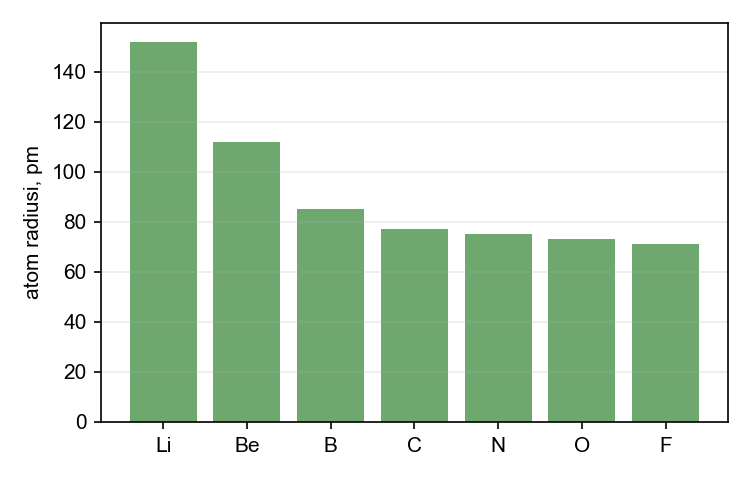
\includegraphics[width=0.86\linewidth]{rasmlar/gen/ra_v08_0.png}\end{center}
Davr bo`yicha chapdan o`ngga atom radiusi qanday o`zgaradi va sababi nima?
\noindent A)~\textsl{Ortadi, qavatlar soni ko`payishi tufayli}\par
\noindent B)~\textsl{Kamayadi, qavatlar soni kamayishi tufayli}\par
\noindent C)~\textsl{O`zgarmaydi}\par
\noindent D)~\textsl{Kamayadi, yadro zaryadi ortishi tufayli}\par
\vspace{4pt}
\noindent\textbf{5.} 0,2 M sirka kislota eritmasida dissotsilanish darajasi 2\% bo`lsa, vodorod ionlari \textbf{konsentratsiyasini (mol/l) aniqlang.}

\noindent A)~\textsl{0,004} \hfill B)~\textsl{0,04} \hfill C)~\textsl{0,0004} \hfill D)~\textsl{0,2}\par
\vspace{4pt}
\noindent\textbf{6.} 33-tartib raqamli element atomida magnit kvant soni m\_l = 1 bo`lgan elektronlardan nechtasining spin kvant soni m\_s = +$\frac{1}{2}$ ga, nechtasiniki m\_s = $-$$\frac{1}{2}$ ga teng?

\noindent A)~\textsl{4 va 3} \hfill B)~\textsl{3 va 4} \hfill C)~\textsl{5 va 3} \hfill D)~\textsl{4 va 4}\par
\vspace{4pt}
\noindent\textbf{7.} FeSO\textsubscript{4}$\cdot$7H\textsubscript{2}O kristallogidratida kristallizatsion suvning massa \textbf{ulushini (\%) aniqlang.}

\noindent A)~\textsl{54,7} \hfill B)~\textsl{45,3} \hfill C)~\textsl{22,7} \hfill D)~\textsl{82,9}\par
\vspace{4pt}
\noindent\textbf{8.} 1 M HCl eritmasining normal \textbf{konsentratsiyasini (n) aniqlang.}

\noindent A)~\textsl{2} \hfill B)~\textsl{0,5} \hfill C)~\textsl{1} \hfill D)~\textsl{1,5}\par
\vspace{4pt}
\noindent\textbf{9.} Zichligi 1,3 g/ml bo`lgan 30\% li HNO\textsubscript{3} eritmasining molyar \textbf{konsentratsiyasini (mol/l) aniqlang.}

\noindent A)~\textsl{0,62} \hfill B)~\textsl{12,38} \hfill C)~\textsl{6,19} \hfill D)~\textsl{4,76}\par
\vspace{4pt}
\end{multicols}
\noindent\textbf{10.} CuSO\textsubscript{4} tuzining eruvchanligi (g/100 g suv) haroratga bog`liq jadvalda keltirilgan:
\begin{center}
\renewcommand{\arraystretch}{1.15}
\begin{tabular}{|c|c|c|c|c|}\hline
\textbf{t, \textdegree{}C} & \textbf{0} & \textbf{20} & \textbf{40} & \textbf{60} \\ \hline
S, g/100 g suv & 15 & 24 & 38 & 60 \\ \hline
\end{tabular}
\end{center}
60 \textdegree{}C da tayyorlangan to`yingan 320 g eritma 0 \textdegree{}C gacha sovitildi. Cho`kmaga tushgan tuz \textbf{massasini (g) aniqlang.}

\noindent A)~\textsl{120} \hfill B)~\textsl{30} \hfill C)~\textsl{180} \hfill D)~\textsl{90}\par
\vspace{4pt}
\begin{multicols}{2}
\noindent\textbf{11.} Kislorod (\textit{Z} = 8) atomida nechta juftlashmagan elektron bor?

\noindent A)~\textsl{2} \hfill B)~\textsl{3} \hfill C)~\textsl{1} \hfill D)~\textsl{4}\par
\vspace{4pt}
\noindent\textbf{12.} pH = 2 bo`lgan kuchli kislota eritmasi 10 marta suyultirildi. Yangi eritmaning pH \textbf{qiymatini aniqlang.}

\noindent A)~\textsl{4} \hfill B)~\textsl{2} \hfill C)~\textsl{3} \hfill D)~\textsl{7}\par
\vspace{4pt}
\noindent\textbf{13.} H\textsubscript{2} + I\textsubscript{2} $\rightleftarrows$ 2HI reaksiyasi 5 l hajmli idishda o`tkazildi. Ma'lumotlar jadvalda berilgan:
\begin{center}
\renewcommand{\arraystretch}{1.15}
\begin{tabular}{|c|c|c|c|}\hline
\textbf{Modda} & \textbf{H\textsubscript{2}} & \textbf{I\textsubscript{2}} & \textbf{HI} \\ \hline
Boshlang`ich, mol & 2 & 6 & 0 \\ \hline
Muvozanatda, mol & --- & --- & 3 \\ \hline
\end{tabular}
\end{center}
H\textsubscript{2} ning necha foizi reaksiyaga \textbf{kirishganini aniqlang.}

\noindent A)~\textsl{37,5} \hfill B)~\textsl{112,5} \hfill C)~\textsl{75} \hfill D)~\textsl{25}\par
\vspace{4pt}
\noindent\textbf{14.} 4Li + O\textsubscript{2} $\to$ 2Li\textsubscript{2}O jarayoni uchun 64 g O\textsubscript{2} olingan. Li\textsubscript{2}O \textbf{massasini (g) aniqlang.}

\noindent A)~\textsl{30} \hfill B)~\textsl{240} \hfill C)~\textsl{120} \hfill D)~\textsl{60}\par
\vspace{4pt}
\noindent\textbf{15.} 0,4 mol Ca(OH)\textsubscript{2} tutgan eritmadan 0,6 mol karbonat angidrid o`tkazildi. Eritmada qolgan kalsiy gidrokarbonatning \textbf{massasini (g) aniqlang.}

\noindent A)~\textsl{40} \hfill B)~\textsl{97,2} \hfill C)~\textsl{20} \hfill D)~\textsl{32,4}\par
\vspace{4pt}
\noindent\textbf{16.} D-metallar va ularning birikmalari haqida qaysi fikrlar to`g`ri? 1) Fe(OH)\textsubscript{2} havoda qo`ng`ir rangga o`tadi; 2) Xrom (VI) oksidi (CrO\textsubscript{3}) kislotali oksid; 3) Rux eritmada Fe\textsuperscript{2+} ni siqib chiqara olmaydi; 4) Cr\textsubscript{2}O\textsubscript{3} asosli oksid

\noindent A)~\textsl{1, 3} \hfill B)~\textsl{1, 4} \hfill C)~\textsl{1, 2} \hfill D)~\textsl{2, 3}\par
\vspace{4pt}
\noindent\textbf{17.} Ca(HCO\textsubscript{3})\textsubscript{2} $\to$ CaCO\textsubscript{3} + CO\textsubscript{2} + H\textsubscript{2}O jarayoni uchun tarkibida 80\% aralashma bo`lgan 81 g namuna (asosiy modda Ca(HCO\textsubscript{3})\textsubscript{2}) olingan. CO\textsubscript{2} \textbf{hajmini (l, n.sh.) aniqlang.}

\noindent A)~\textsl{2,24} \hfill B)~\textsl{4,48} \hfill C)~\textsl{1,12} \hfill D)~\textsl{3,36}\par
\vspace{4pt}
\noindent\textbf{18.} CaO + CO\textsubscript{2} $\to$ CaCO\textsubscript{3} jarayoni uchun 4,48 l (n.sh.) CO\textsubscript{2} olingan. CaCO\textsubscript{3} \textbf{miqdorini (mol) aniqlang.}

\noindent A)~\textsl{0,4} \hfill B)~\textsl{0,2} \hfill C)~\textsl{0,1} \hfill D)~\textsl{0,3}\par
\vspace{4pt}
\noindent\textbf{19.} Ca $\to$ ? $\to$ ? $\to$ ? o`zgarishlar zanjirida (reagentlar: O\textsubscript{2}, H\textsubscript{2}O, CO\textsubscript{2}) 1-bosqichda hosil bo`ladigan modda \textbf{formulasini toping.}

\noindent A)~\textsl{NaCl} \hfill B)~\textsl{K\textsubscript{3}PO\textsubscript{4}} \hfill C)~\textsl{CaO} \hfill D)~\textsl{H\textsubscript{2}SO\textsubscript{3}}\par
\vspace{4pt}
\noindent\textbf{20.} 0,1 mol metan xlor bilan to`liq xlorlanib, CCl\textsubscript{4} olindi. Sarflangan xlor \textbf{hajmini (l, n.sh.) aniqlang.}

\noindent A)~\textsl{2,24} \hfill B)~\textsl{8,96} \hfill C)~\textsl{4,48} \hfill D)~\textsl{6,72}\par
\vspace{4pt}
\noindent\textbf{21.} Etilen va asetilendan iborat 8 g aralashmani to`liq gidrogenlash uchun sarflanadigan vodorod \textbf{hajmini (l, n.sh.) aniqlang.}

\noindent A)~\textsl{22,4} \hfill B)~\textsl{5,6} \hfill C)~\textsl{6,72} \hfill D)~\textsl{11,2}\par
\vspace{4pt}
\noindent\textbf{22.} 6,5 g C\textsubscript{2}H\textsubscript{2} dan quyidagi ikki bosqichda CH\textsubscript{3}COOH olinadi: 1) C\textsubscript{2}H\textsubscript{2} + H\textsubscript{2}O $\to$ CH\textsubscript{3}CHO (unum 50\%); 2) CH\textsubscript{3}CHO + Ag\textsubscript{2}O $\to$ CH\textsubscript{3}COOH + 2Ag (unum 90\%). Oxirgi mahsulot CH\textsubscript{3}COOH ning \textbf{massasini (g) toping.}

\noindent A)~\textsl{13,5} \hfill B)~\textsl{7,5} \hfill C)~\textsl{15} \hfill D)~\textsl{6,75}\par
\vspace{4pt}
\noindent\textbf{23.} C\textsubscript{2}H\textsubscript{5}OH va CH\textsubscript{3}OH dan iborat 12,4 g aralashma natriy bilan to`liq reaksiyaga kirishganda ajraladigan vodorod \textbf{hajmini (l, n.sh.) toping.}

\noindent A)~\textsl{6,72} \hfill B)~\textsl{1,68} \hfill C)~\textsl{3,36} \hfill D)~\textsl{1,78}\par
\vspace{4pt}
\noindent\textbf{24.} 1,5 g metanal Ag\textsubscript{2}O ning ammiakli eritmasi bilan to`liq oksidlanganda hosil bo`lgan kumush \textbf{massasini (g) aniqlang.}

\noindent A)~\textsl{21,6} \hfill B)~\textsl{5,4} \hfill C)~\textsl{43,2} \hfill D)~\textsl{10,8}\par
\vspace{4pt}
\noindent\textbf{25.} C\textsubscript{3}H\textsubscript{9}N aminlarning izomerlari soni nechta?

\noindent A)~\textsl{5} \hfill B)~\textsl{4} \hfill C)~\textsl{3} \hfill D)~\textsl{6}\par
\vspace{4pt}
\noindent\textbf{26.} Murakkab efirlar va yog`lar haqida qaysi fikrlar to`g`ri? 1) Etilatsetat efir hidli suyuqlik; 2) Yog`lar glitserin va yuqori yog` kislotalarning murakkab efirlari; 3) Murakkab efirlarning gidrolizi ishqoriy muhitda qaytmas; 4) Suyuq yog`larni gidrogenlab qattiq yog` olinadi

\noindent\begin{tabular}{@{}p{0.47\linewidth}@{}p{0.47\linewidth}@{}}
A)~\textsl{1, 2, 3} & B)~\textsl{1, 3, 4} \\
C)~\textsl{1, 2, 4} & D)~\textsl{1, 2, 3, 4} \\
\end{tabular}\par
\vspace{4pt}
\noindent\textbf{27.} Rasmda siklik uglevodorodning tuzilish formulasi berilgan.
\begin{center}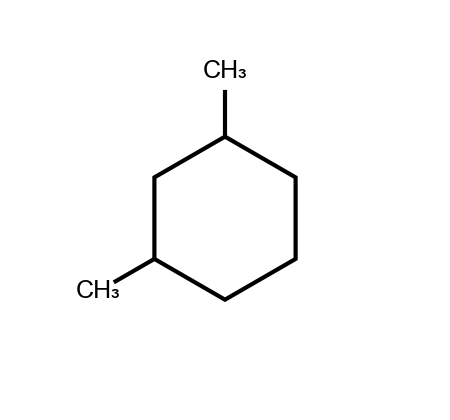
\includegraphics[width=0.86\linewidth]{rasmlar/gen/rn_397205.png}\end{center}
Birikmaning \textbf{nomini toping.}

\noindent\begin{tabular}{@{}p{0.47\linewidth}@{}p{0.47\linewidth}@{}}
A)~\textsl{1,3-dimetilsiklogeksan} & B)~\textsl{1,3-dimetilsiklopentan} \\
C)~\textsl{metilsiklopentan} & D)~\textsl{1,2-dimetilsiklogeksan} \\
\end{tabular}\par
\vspace{4pt}
\noindent\textbf{28.} 22,5 g glitsin HCl bilan reaksiyaga kirishganda hosil bo`lgan tuz \textbf{massasini (g) aniqlang.}

\noindent A)~\textsl{33,45} \hfill B)~\textsl{22,5} \hfill C)~\textsl{10,95} \hfill D)~\textsl{66,9}\par
\vspace{4pt}
\noindent\textbf{29.} 6,5 g C\textsubscript{2}H\textsubscript{2} dan quyidagi ikki bosqichda C\textsubscript{2}H\textsubscript{4}Br\textsubscript{2} olinadi: 1) C\textsubscript{2}H\textsubscript{2} + H\textsubscript{2} $\to$ C\textsubscript{2}H\textsubscript{4} (unum 80\%); 2) C\textsubscript{2}H\textsubscript{4} + Br\textsubscript{2} $\to$ C\textsubscript{2}H\textsubscript{4}Br\textsubscript{2} (unum 75\%). Oxirgi mahsulot C\textsubscript{2}H\textsubscript{4}Br\textsubscript{2} ning \textbf{massasini (g) toping.}

\noindent A)~\textsl{35,25} \hfill B)~\textsl{37,6} \hfill C)~\textsl{47} \hfill D)~\textsl{28,2}\par
\vspace{4pt}
\end{multicols}
\noindent\textbf{30.} Uch probirkada (\textit{X}, \textit{Y}, \textit{Z}) fenol, glitserin, formalin eritmalari bor (tartibsiz). Ularga FeCl\textsubscript{3} va Cu(OH)\textsubscript{2} ta'sir ettirildi. Kuzatuvlar jadvalda:
\begin{center}
\renewcommand{\arraystretch}{1.15}
\begin{tabular}{|c|c|c|}\hline
\textbf{Probirka} & \textbf{FeCl\textsubscript{3}} & \textbf{Cu(OH)\textsubscript{2}} \\ \hline
\textit{X} & o`zgarish yo`q & tiniq ko`k eritma \\ \hline
\textit{Y} & o`zgarish yo`q & qizdirilganda qizil cho`kma \\ \hline
\textit{Z} & binafsha rang & --- \\ \hline
\end{tabular}
\end{center}
\textit{X}, \textit{Y}, \textit{Z} probirkalardagi \textbf{moddalarni aniqlang.}
\noindent A)~\textsl{\textit{X} -- glitserin, \textit{Y} -- formalin, \textit{Z} -- fenol}\par
\noindent B)~\textsl{\textit{X} -- glitserin, \textit{Y} -- fenol, \textit{Z} -- formalin}\par
\noindent C)~\textsl{\textit{X} -- fenol, \textit{Y} -- formalin, \textit{Z} -- glitserin}\par
\noindent D)~\textsl{\textit{X} -- fenol, \textit{Y} -- glitserin, \textit{Z} -- formalin}\par
\vspace{4pt}
\begin{multicols}{2}
\noindent\textbf{31.} Rasmda aralashmani ajratish usuli ko`rsatilgan. Bu usul nima deb ataladi?
\begin{center}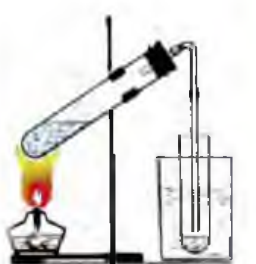
\includegraphics[width=0.86\linewidth]{rasmlar/darslik/d_distill.png}\end{center}

\noindent\begin{tabular}{@{}p{0.47\linewidth}@{}p{0.47\linewidth}@{}}
A)~\textsl{bug`latish} & B)~\textsl{dekantatsiya} \\
C)~\textsl{filtrlash} & D)~\textsl{distillash} \\
\end{tabular}\par
\vspace{4pt}
\noindent\textbf{32.} Kimyo laboratoriyasida ishlash qoidalari haqida qaysi fikrlar to`g`ri? 1) Suvni konsentrlangan kislotaga tez quyish mumkin; 2) Ishqor teriga tushsa, qo`l suv bilan yuviladi; 3) Kimyoviy moddalar hidini bevosita nafas olib aniqlash kerak; 4) Ortiqcha reaktiv idishga qaytariladi

\noindent\begin{tabular}{@{}p{0.47\linewidth}@{}p{0.47\linewidth}@{}}
A)~\textsl{4} & B)~\textsl{2} \\
C)~\textsl{3} & D)~\textsl{1, 3   ---} \\
\end{tabular}\par
\vspace{4pt}
\end{multicols}
\medskip
\noindent\setlength{\fboxsep}{0pt}\fbox{\begin{tabular}{p{0.74\linewidth}|p{0.2\linewidth}}
\parbox[t]{0.72\linewidth}{\vspace{3pt}\textbf{Topshiriqlar (33--35) va javob variant (A--F)larini o`zaro to`g`ri moslashtiring.} CaCO\textsubscript{3} va Na\textsubscript{2}CO\textsubscript{3} dan iborat 41,2 g aralashma mo`l xlorid kislota bilan reaksiyaga kirishdi. Ajralgan gaz 0,6 mol NaOH tutgan eritmadan o`tkazildi.
\vspace{3pt}} & \parbox[t]{0.19\linewidth}{\vspace{3pt}A~\textsl{0,8}\\[3pt]
B~\textsl{17,92}\\[3pt]
C~\textsl{13,44}\\[3pt]
D~\textsl{8,96}\\[3pt]
E~\textsl{1,6}\\[3pt]
F~\textsl{6,72}}\\ \hline
\parbox[t]{0.72\linewidth}{\vspace{2pt}\textbf{33. Ajralgan gazning hajmini (l, n.sh.) aniqlang.}\vspace{2pt}} & \\ \hline
\parbox[t]{0.72\linewidth}{\vspace{2pt}\textbf{34. Aralashmani to`liq eritish uchun sarflangan HCl miqdorini (mol) aniqlang.}\vspace{2pt}} & \\ \hline
\parbox[t]{0.72\linewidth}{\vspace{2pt}\textbf{35. Gaz NaOH eritmasidan o`tkazilganda hosil bo`lgan tuz (NaHCO\textsubscript{3}) massasini (g) aniqlang (reaksiya unumi 80\%).}\vspace{2pt}} & 
\end{tabular}}
\par\bigskip
\noindent\textbf{36.} KMnO\textsubscript{4} + KI + H\textsubscript{2}SO\textsubscript{4} $\to$ MnSO\textsubscript{4} + I\textsubscript{2} + K\textsubscript{2}SO\textsubscript{4} + H\textsubscript{2}O reaksiya tenglamasini tenglang. Reagentlar (chap qism) koeffitsiyentlari \textbf{yig`indisini toping.}
\javob
\noindent\textbf{37.} Ketma-ket ulangan ikkita elektrolizyordan (CuSO\textsubscript{4} va AgNO\textsubscript{3} eritmalari, inert elektrodlar) tok o`tkazildi. Birinchi elektrolizyor katodida 12,8 g mis ajraldi. Ikkala elektrolizyor anodlarida ajralgan kislorodning umumiy \textbf{hajmini (l, n.sh.) toping} (anodda ikkalasida ham O\textsubscript{2} ajraladi).
\javob
\noindent\textbf{38.} 10 m\textsuperscript{3} suvda Ca(HCO\textsubscript{3})\textsubscript{2} konsentratsiyasi 10 mol/m\textsuperscript{3}, Mg(HCO\textsubscript{3})\textsubscript{2} niki 10 mol/m\textsuperscript{3}. Suvni Ca(OH)\textsubscript{2} bilan to`liq yumshatish uchun Ca(OH)\textsubscript{2} ning \textbf{massasini (kg) hisoblang.}
\javob
\noindent\textbf{39.} 9,4 g fenoldan 2,4,6-tribromfenol olishda unum 60\% bo`lsa, mahsulot \textbf{massasini (g) aniqlang} (boshlang`ich modda massasi 9,4 g).
\javob
\noindent\textbf{40.} Polimerlanish darajasi 2000 bo`lgan polistirol ning 208 g namunasini olish uchun polimerlanish unumi 90\% bo`lganda qancha monomer (C\textsubscript{8}H\textsubscript{8}) kerak (g)?
\javob
\par\bigskip\begin{center}\textbf{\fontsize{13}{15}\selectfont YOZMA ISH}\end{center}
\noindent\textbf{41.} \textbf{Topshiriqni bajarish jarayonida barcha reaksiya tenglamalarini yozing. Miqdoriy va arifmetik hisoblashlarni (unga asos bo`lgan usul yoki formulani ko`rsatgan holda) uzviy ketma-ketlikda bajaring.}\par\smallskip
Hajmi 10 l bo`lgan idishda 2NO + O\textsubscript{2} $\rightleftarrows$ 2NO\textsubscript{2} sistema muvozanat holatiga keldi. Muvozanat qaror topganda idishdagi moddalar miqdori: NO -- 2,5 mol, O\textsubscript{2} -- 2,75 mol; NO\textsubscript{2} -- 0,5 mol.\par
\noindent 1)Muvozanat konstantasini (K) hisoblang.\par
\noindent 2)Moddalarning boshlang`ich konsentratsiyalarini (mol/l) aniqlang. Boshlang`ich moddalarning umumiy miqdorini (mol) ham toping.\par
\noindent 3)NO ning necha foizi reaksiyaga kirishgan?\par
\noindent 4)Idish hajmi izotermik ravishda 2 marta kamaytirilsa, to`g`ri reaksiya tezligi (elementar reaksiya deb hisoblang) necha marta o`zgaradi? Teskari reaksiya uchun K' = 1/K ni ham hisoblang.\par
\noindent 5)Bosim oshirilganda muvozanat qaysi tomonga siljiydi va K qiymati qanday o`zgaradi? Muvozanatdagi umumiy mol miqdorining boshlang`ich mol miqdoriga nisbatini toping. Muvozanat aralashmasining o`rtacha molyar massasini (g/mol) ham hisoblang.\par
\diqqat{Mazkur topshiriq kengaytirilgan javobni talab etib, uning yechilish usuli va shu usul asosidagi barcha hisoblash amallari javoblar varaqasida aks etishi lozim.}
\noindent\textbf{42.} Quyidagi o`zgarishlar zanjirida \textit{X}, \textit{Y}, \textit{Z} noma'lum organik moddalar:\par
\[\setlength{\fboxsep}{0pt}\text{CH\textsubscript{3}COOC\textsubscript{2}H\textsubscript{5}}\xrightarrow{\text{NaOH}}\text{\textit{X}}\xrightarrow{\text{NaOH (suyuqlanma), t\textdegree{}}}\text{\textit{Y}}\xrightarrow{\text{Cl\textsubscript{2}, yorug`lik}}\text{CH\textsubscript{3}Cl}\]
\noindent 1)CH\textsubscript{3}COOC\textsubscript{2}H\textsubscript{5} $\to$ \textit{X} : reaksiya tenglamasini yozing; hosil bo`lgan moddani nomlang.\par
\noindent 2)\textit{X} $\to$ \textit{Y} : reaksiya tenglamasini yozing; hosil bo`lgan moddani nomlang.\par
\noindent 3)\textit{Y} $\to$ CH\textsubscript{3}Cl : reaksiya tenglamasini yozing; hosil bo`lgan moddani nomlang.\par
\diqqat{Mazkur topshiriq kengaytirilgan javobni talab etib, uning yechilish usuli va shu usul asosidagi barcha hisoblash amallari javoblar varaqasida aks etishi lozim.}
\noindent\textbf{43.} \textbf{Topshiriqni bajarish jarayonida barcha reaksiya tenglamalarini yozing. Miqdoriy va arifmetik hisoblashlarni (unga asos bo`lgan usul yoki formulani ko`rsatgan holda) uzviy ketma-ketlikda bajaring.}\par\smallskip
75,2 g Cu(NO\textsubscript{3})\textsubscript{2} qizdirilganda qisman parchalandi va qattiq qoldiq massasi 64,4 g bo`ldi. Ajralgan gazlar aralashmasi 200 g suvga to`liq yuttirildi. Qattiq qoldiq esa CuO ni to`liq eritadigan (ortiqcha bo`lmagan) miqdordagi suyultirilgan H\textsubscript{2}SO\textsubscript{4} da eritildi, hosil bo`lgan eritmaga temir qipig`i solindi.\par
\noindent 1)Parchalanish reaksiyasi tenglamasini yozing. Parchalangan Cu(NO\textsubscript{3})\textsubscript{2} ning ulushini (\%) va ajralgan gazlar hajmini (l, n.sh.) aniqlang.\par
\noindent 2)Qattiq qoldiqdagi CuO ning massa ulushini (\%) hisoblang.\par
\noindent 3)Gazlar suvga yuttirilganda hosil bo`lgan eritmadagi HNO\textsubscript{3} ning massa ulushini (\%) toping (reaksiya tenglamasini yozing).\par
\noindent 4)Temir qipig`i eritmadagi barcha Cu\textsuperscript{2+} ionlarini siqib chiqarishi uchun zarur temir massasini (g) va ajralgan mis massasini (g) aniqlang (reaksiya tenglamalarini yozing).\par
\noindent 5)Ajralgan NO\textsubscript{2} va O\textsubscript{2} gazlari aralashmasining o`rtacha molyar massasini (g/mol) hisoblang.\par
\diqqat{Mazkur topshiriq kengaytirilgan javobni talab etib, uning yechilish usuli va shu usul asosidagi barcha hisoblash amallari javoblar varaqasida aks etishi lozim.}
\newpage
\noindent\textbf{\fontsize{13}{15}\selectfont Nazorat testi}\ \textit{$\cdot$ 8-variant}\hfill \textbf{Javoblar kaliti}\par\smallskip\hrule\smallskip
\textit{Faqat o`qituvchi uchun.}\par\medskip
\noindent\textbf{1--32-savollar}\par\smallskip
\noindent\begin{tabular}{|c|c|c|c|c|c|c|c|c|c|c|c|c|c|c|c|}\hline
\textbf{1} & \textbf{2} & \textbf{3} & \textbf{4} & \textbf{5} & \textbf{6} & \textbf{7} & \textbf{8} & \textbf{9} & \textbf{10} & \textbf{11} & \textbf{12} & \textbf{13} & \textbf{14} & \textbf{15} & \textbf{16}\\\hline
\textsl{B} & \textsl{B} & \textsl{B} & \textsl{D} & \textsl{A} & \textsl{A} & \textsl{B} & \textsl{C} & \textsl{C} & \textsl{D} & \textsl{A} & \textsl{C} & \textsl{C} & \textsl{C} & \textsl{D} & \textsl{C}\\\hline
\textbf{17} & \textbf{18} & \textbf{19} & \textbf{20} & \textbf{21} & \textbf{22} & \textbf{23} & \textbf{24} & \textbf{25} & \textbf{26} & \textbf{27} & \textbf{28} & \textbf{29} & \textbf{30} & \textbf{31} & \textbf{32}\\\hline
\textsl{A} & \textsl{B} & \textsl{C} & \textsl{B} & \textsl{D} & \textsl{D} & \textsl{C} & \textsl{A} & \textsl{B} & \textsl{D} & \textsl{A} & \textsl{A} & \textsl{D} & \textsl{A} & \textsl{D} & \textsl{B}\\\hline
\end{tabular}\par\medskip
\noindent\textbf{33--35-savollar}\par\smallskip
\noindent\begin{tabular}{|c|c|c|}\hline \textbf{No} & \textbf{Javob} & \textbf{Qiymat}\\\hline
33 & \textsl{D} & 8,96\\\hline
34 & \textsl{A} & 0,8\\\hline
35 & \textsl{C} & 13,44\\\hline
\end{tabular}\par\medskip
\noindent\textbf{36--40-savollar}\par\smallskip
\noindent\begin{tabular}{|c|c|}\hline \textbf{No} & \textbf{To`g`ri javob}\\\hline
36 & 20\\\hline
37 & 4,48\\\hline
38 & 22,2\\\hline
39 & 19,86\\\hline
40 & 231,11\\\hline
\end{tabular}\par\medskip
\noindent\textbf{41--43-topshiriqlar: qisqa yechim}\par\smallskip
\noindent\textbf{41-topshiriq.}\par
\noindent 1) K = [NO\textsubscript{2}]\textasciicircum{}2/([NO]\textasciicircum{}2$\cdot$[O\textsubscript{2}]) = \textbf{0,145}\par
\noindent 2) n(bosh.) = n(muv.) + n(sarflangan): NO 0,3, O\textsubscript{2} 0,3 mol/l; n(bosh.) = \textbf{6 mol}\par
\noindent 3) $\alpha$ = 0,5/3 = \textbf{16,7\%}\par
\noindent 4) v = k$\cdot$[NO]\textasciicircum{}2$\cdot$[O\textsubscript{2}]; hajm 2 marta kamayganda konsentratsiyalar 2 marta ortadi: 2\textasciicircum{}3 = \textbf{8 marta ortadi}; K' = \textbf{6,875}\par
\noindent 5) $\Delta$n = -1 $\to$ muvozanat o`ngga siljiydi; K harorat funksiyasi, o`zgarmaydi. n(muv.)/n(bosh.) = 5,75/6 = \textbf{0,958}; M(o`rt.) = $\Sigma$(n$\cdot$M)/$\Sigma$n = \textbf{32,35 g/mol}\par
\noindent Jami: M 15 + A 10 = 25 ball.\par
\noindent\textbf{42-topshiriq.}\par
\noindent 1) CH\textsubscript{3}COOC\textsubscript{2}H\textsubscript{5} + NaOH $\to$ CH\textsubscript{3}COONa (natriy atsetat)\par
\noindent 2) CH\textsubscript{3}COONa + NaOH (suyuqlanma), t\textdegree{} $\to$ CH\textsubscript{4} (metan)\par
\noindent 3) CH\textsubscript{4} + Cl\textsubscript{2}, yorug`lik $\to$ CH\textsubscript{3}Cl (xlormetan)\par
\noindent Jami 25 ball.\par
\noindent\textbf{43-topshiriq.}\par
\noindent 1) 2Cu(NO\textsubscript{3})\textsubscript{2} $\xrightarrow{\text{t}}$ 2CuO + 4NO\textsubscript{2} + O\textsubscript{2}. Massa kamayishi 75,2 $-$ 64,4 = 10,8 g; 2 mol (376 g) parchalanganda 216 g kamayadi $\to$ parchalangan 0,1 mol; boshlang`ich 0,4 mol $\to$ \textbf{25\%}; gazlar NO\textsubscript{2} 0,2 + O\textsubscript{2} 0,05 mol $\to$ \textbf{5,6 l}\par
\noindent 2) CuO 0,1 mol = 8 g; $\omega$ = 8/64,4 = \textbf{12,4\%}\par
\noindent 3) 4NO\textsubscript{2} + O\textsubscript{2} + 2H\textsubscript{2}O $\to$ 4HNO\textsubscript{3}: HNO\textsubscript{3} 0,2 mol = 12,6 g; eritma 200 + 9,2 + 1,6 = 210,8 g $\to$ \textbf{5,98\%}\par
\noindent 4) CuO + H\textsubscript{2}SO\textsubscript{4} $\to$ CuSO\textsubscript{4} + H\textsubscript{2}O (0,1 mol); eritmada Cu\textsuperscript{2+}: Cu(NO\textsubscript{3})\textsubscript{2} 0,3 + CuSO\textsubscript{4} 0,1 = 0,4 mol; Fe + Cu\textsuperscript{2+} $\to$ Fe\textsuperscript{2+} + Cu: Fe \textbf{22,4 g}, Cu \textbf{25,6 g}\par
\noindent 5) NO\textsubscript{2} : O\textsubscript{2} = 4 : 1 $\to$ M = (4$\cdot$46 + 32)/5 = \textbf{43,2 g/mol}\par
\noindent Jami: M 15 + A 10 = 25 ball.\par
\par\bigskip\noindent\textbf{Mavzular taqsimoti}\par\smallskip
{\small\noindent\begin{longtable}{|c|p{7.2cm}|p{5.4cm}|c|}\hline \textbf{No} & \textbf{Mavzu} & \textbf{Tekshiriladigan ko`nikma} & \textbf{Ball}\\\hline
1 & 7-sinf (jism va modda) & Bilim va tushunish & 1\\\hline
2 & 8-sinf (Gey-Lyussak, Avogadro) & Hisoblash va masala yechish & 1\\\hline
3 & 8-sinf (Gey-Lyussak, Avogadro) & Hisoblash va masala yechish & 1\\\hline
4 & 8-sinf (davriy qonun, diagramma) & Grafik tahlili & 1\\\hline
5 & 9-sinf; Tirkashev IV bob (dissotsilanish darajasi) & Hisoblash va masala yechish & 1\\\hline
6 & Tirkashev I bob (kvant sonlari) & Bilim va tushunish & 1\\\hline
7 & 7-sinf; Tirkashev (kristallogidrat) & Hisoblash va masala yechish & 1\\\hline
8 & 11-sinf 4-bob (normal konsentratsiya) & Hisoblash va masala yechish & 1\\\hline
9 & 11-sinf 4-bob (molyar konsentratsiya) & Hisoblash va masala yechish & 1\\\hline
10 & Tirkashev III bob (eruvchanlik, jadval) & Jadval tahlili & 1\\\hline
11 & Tirkashev I bob; 8-sinf (elektron konfiguratsiya) & Bilim va tushunish & 1\\\hline
12 & 9-sinf; Tirkashev IV bob (pH) & Hisoblash va masala yechish & 1\\\hline
13 & Tirkashev VI bob (muvozanat, jadval) & Jadval tahlili & 1\\\hline
14 & 9-sinf; Tirkashev (IA metallar, hisob) & Hisoblash va masala yechish & 1\\\hline
15 & 9-sinf (uglerod; suv qattiqligi) & Hisoblash va masala yechish & 1\\\hline
16 & 9-sinf; Tashev (Fe, Cu, Zn, Cr) & Bilim va tushunish & 1\\\hline
17 & 9-sinf; Tirkashev (suv qattiqligi, hisob) & Hisoblash va masala yechish & 1\\\hline
18 & 9-sinf; Tirkashev (oksid/asos/kislota/tuz, hisob) & Hisoblash va masala yechish & 1\\\hline
19 & 8-sinf; 9-sinf (genetik bog`lanish) & Bilim va tushunish & 1\\\hline
20 & 10-sinf \S{}8 (alkanlar galogenlanishi) & Hisoblash va masala yechish & 1\\\hline
21 & 10-sinf \S{}13, \S{}15 (alken va alkin birikish reaksiyalari) & Hisoblash va masala yechish & 1\\\hline
22 & 10-sinf (ikki bosqichli hisob) & Hisoblash va masala yechish & 1\\\hline
23 & 10-sinf \S{}21 (spirtlar) & Hisoblash va masala yechish & 1\\\hline
24 & 10-sinf \S{}24; \S{}26; \S{}30 (kumush ko`zgu) & Hisoblash va masala yechish & 1\\\hline
25 & 10-sinf \S{}6, \S{}12, \S{}20, \S{}28 (izomeriya) & Bilim va tushunish & 1\\\hline
26 & 10-sinf (mavzuga oid paragraflar); Abdusamatov & Bilim va tushunish & 1\\\hline
27 & 10-sinf (sikloalkanlar) & Rasm bo`yicha tahlil & 1\\\hline
28 & 10-sinf \S{}34 & Hisoblash va masala yechish & 1\\\hline
29 & 10-sinf (ikki bosqichli hisob) & Hisoblash va masala yechish & 1\\\hline
30 & 7--10-sinf va Tashev (laboratoriya ishlari, sifat reaksiyalar) & Jadval tahlili & 1\\\hline
31 & 7-sinf (13-rasm) & Rasm bo`yicha tahlil & 1\\\hline
32 & 7-sinf (xavfsizlik qoidalari); 10-sinf lab. & Bilim va tushunish & 1\\\hline
33--35 & Aralash masala (moslashtirish) & Ko`p bosqichli hisob & 3\\\hline
36--40 & Qisqa javobli masalalar & Hisoblash & 5\\\hline
41--43 & Yozma ish & Usul va hisob (M, A) & 75\\\hline
\end{longtable}}
\end{document}
